\section{Sphinx Packet Format}

HOPR uses the SPHINX packet format \cite{sphinxpaper} to encapsulate and route data packets in order to achieve sender and receiver unlinkability. The SPHINX packet format determines how mixnet packet are created and transformed in order to relay them to the next downstream node. Each sphinx packet consists of two parts:

\begin{figure}[H]
    \centering
    \begin{tabular}{| c |}
        \hline
        \\[-0.8em]
        Header                                       \\[0.2em]
        \begin{tabular}{| m{0.27\textwidth} | m{0.27\textwidth} | m{0.27\textwidth} |}
            \hline
            Key derivation $\alpha$ & encrypted routing information $\beta$ & integrity tag $\gamma$ \\
            \hline
        \end{tabular}                    \\[0.9em]
        \hline
        \hline
        \\[-0.7em]
        Padded and Onion encrypted payload  $\delta$ \\[0.7em]
        \hline
    \end{tabular}
    \label{fig:Sphinx packet format}
    \caption{Sphinx packet format}
\end{figure}

\subsection{Construction}
We will explain in the following all the steps a sphinx packet goes through in order to arrive to its final destination starting from the key derivation in order to extract new shared keys with all the relay nodes to unblinding the routing information using those shared keys in order to find the public key of the next relay node and checking the routing information's integrity before sending it. Each node then deletes that information and replaces it with their own blinding and decrypts one layer of the payload which has several layers of encryption similar to onion routing.
\paragraph{Notation:}Let $\kappa=128$ be the security parameter. An adversary will have to do about $2^\kappa$ operations to break the security of Sphinx with non negligible probability.
Let $r$ be the maximum number of nodes that a Sphinx mix message will traverse before being delivered to its destination.
\\$G$ is a prime order cyclic group satisfying the Decisional Diffie-Hellman Assumption, we use the secp256k1 elliptic curve \cite{sec2}. The element $g$ is a generator of $G$ and $q$ is the (prime) order of $G$, with $q\approx2^{\kappa}$.
$G^*$is the set of non-identity elements of G. $h_b$ is a pre-image resistant hash function used to compute blinding factors and modeled as a random oracle such that:
$h_b:G^*\times G^*\rightarrow\mathbb{Z}^*_q$ where $\mathbb{Z}^*_q$ is the field of non-identity elements of $\mathbb{Z}_q$ (field of integers). We use the BLAKE2s hash function \cite{blake2}.
    \\~\\Each node $n$ has a private key $x_n\in \mathbb{Z}^*_q$ and a public key $y_n=g^{x_n}\in G^*$.
    The $\alpha_i$ are the group elements which, when combined with the nodes’ public keys, allow computing a shared key for each via Diffie-Hellman (DH) key exchange, and so the first node in the user-chosen route can forward the packet to the next, and only that mix-node can decrypt it.
    The $s_i$ are the DH shared secrets, $b_i$ are the blinding factors.

    \paragraph{Key derivation}
    The sender $(A)$ picks a random $x\in \mathbb{Z}^*_q$ that is used to derive new keys for every packet.
    \newline $(A)$ randomly picks a path consisting of intermediate nodes $(B)$, $(C)$,$(D)$ and the final destination of the packet $(Z)$.
    \newline $(A)$ performs an offline Diffie-Hellman key exchange with each of these nodes and derives shared keys with each of them.
    \newline $(A)$ computes a sequence of $r$ tuples (in our case r=4)  $$(\alpha_0,s_0,b_0),.................,(\alpha_{r-1},s_{r-1},b_{r-1})$$ as follows:
    \begin{itemize}
        \item $\alpha_0=g^x,s_0=y^x_B,b_0=h_b(a_0,s_0)$
        \item $\alpha_1=g^{xb_0},s_1=y^{xb_0}_C,b_1=h_b(a_1,s_1)$
        \item $\alpha_2=g^{xb_0b_1},s_2=y^{xb_0b_1}_D,b_2=h_b(a_2,s_2)$
        \item $\alpha_3=g^{xb_0b_1b_2},s_3=y^{xb_0b_1b_2}_D,b_3=h_b(a_3,s_3)$
    \end{itemize}
    Where $y_B,y_C,y_D,y_Z$ are the public keys of the nodes $B,C, D$  which we assume to be available to $A$ .
    \paragraph{Routing information}
    Each node on the path needs to know the next downstream node. Therefore, the sender $(A)$ generates routing information $\beta_i$ for $(B)$, $(C)$ and $(D)$ as well as message $END$ to tell $(Z)$ that it is the final receiver of the message. The END message is a distinguished prefix byte that's added to the final receiver's Ethereum address. The serialization concatenates the $x$ and $y$ coordinates of the public key as follow:
    $$02 + x-coordinate (16\; bytes) + y-coordinate (16\; bytes) if\; y \;is \;even$$
    or $$03 + x-coordinate (16\; bytes) + y-coordinate (16\; bytes) if\; y \;is \;odd$$
The routing information looks as the following:
    $$\beta_{v-1}=(Z\|0_{(2(r-v)+2)\kappa-|Z|}\oplus \rho(h_{\rho}(s_{v-1}))_{[ \,0....(2(r-v)+3)\kappa-1\,]})\|\phi_{v-1}$$
    and
    $$\beta_i=n_{i+1}\|\gamma_{i+1}\|\beta_{{i+1}_{[ \,0....(2r-1)\kappa-1\,] }}\oplus \rho(h_{\rho}(s_{i}))_{[ \,0....(2r+1)\kappa-1\,]} $$ for $0\le i < v-1$ 
    \\~\\Such that $Z$ is the destination's public key and $|Z|$ is its length. $\rho$ is a pseudo-random generator (PRG) and $h_{\rho}$ is the hash function used to key $\rho$.
    $v\leq r$ is the length of the path traversed by the packet where $|Z| \leq (2(r - v) + 2)$. $\phi$ is a filler string such that
    $$\phi_i=\{ \phi_{i-1}\|0_{2\kappa}\}\oplus \rho(h_{\rho}(s_{i-1}))_{[ \,(2(r-i)+3)\kappa..(2r+3)\kappa-1\,]}$$ where $\phi_0=\epsilon$ is an empty string.
    \\$\phi_i$ is generated using the shared secret $s_{i-1}$ and used to ensure the header packets remain constant in size as layers of encryption are added or removed. Upon receiving a packet, the processing node extracts the information destined for it from the route information and the per-hop payload. The extraction is done by deobfuscating and left-shifting the field. This would make the field shorter at each hop, allowing an attacker to deduce the route length. For this reason, the field is pre-padded before forwarding. Since the padding is part of the HMAC, the origin node will have to pre-generate an identical padding (to that which each hop will generate) in order to compute the HMACs correctly for each hop.
    \\~\\$\beta_i$ is computed as the concatenation of $Z$ and a sequence of padding which is then encrypted by XORing with the output of a pseudo-random number generator seeded with shared key $s_{v-1}$ of node $v-1$. The result is finally concatenated with $\phi$ to ensure the header packets remain constant in size.
    \\In the original sphinx paper, $Z$ is concatenated with an identifier $I$ and $0$ padding sequence where $I$ is used for SURBs (Single-Use-Reply Blocks) such that $I \in \{0, 1\}^\kappa$. We don't use $I$ since we don't currently use SURBs .
    \\~\\Since $(A)$ has a shared secret with each of the nodes along the path, it is able to derive blindings for each of them.
    \newline Each node along the path receives an authentication tag $\gamma_i$ in the form of a message authentication code (MAC)
which is encoded in the header.
\newline Some padding is added at each mix stage in order to keep the length of the message invariant at each hop.
\\~\\The mix header is constructed as follow: $$M_i=(\alpha_i,\beta_i,\gamma_i)$$
\newline $(A)$ sends the mix header $M_0$ to $(B)$. Once $(B)$ receives the packet, it derives the shared key $s_0$ by computing $$s_0=(\alpha_0)^b=(g^x)^b=(g^b)^x=y^x_B$$ and removes its blindings. This allows $(B)$ to unblind the routing info that tells $(B)$ the public key of the next downstream node $(C)$.
\paragraph{Integrity check}
By using the derived shared secret $s_i$, each node is able to recompute the authentication tag and check the integrity of the received packet as follows: $$\gamma_i=HMAC(s_i,\beta_i)$$
$(B)$ computes the keyed-hash of the encrypted routing information $\beta_0$ as $$\gamma_0=HMAC(s_0,\beta_0)$$ and compares with the integrity tag $\gamma_0$ attached in the packet header. If the integrity check fails because the header has been tampered with, the packet is dropped. Otherwise, the mix-node proceeds to the next step.
\\This integrity check allows to verify whether or not the header was modified.

\paragraph{Unblinding}
The unblinding works as follow:
\\$(B)$ decrypts the attached $\beta_0$ in order to extract the routing instructions. First, $(B)$ appends a zero-byte padding at the end of $\beta_0$ and decrypts the padded block of routing information $B$ by XORing it with $PRNG(s_{0})$ as follows:
$$(\beta_0\|0_{2\kappa})\oplus \rho(h_{\rho}(s_{0}))$$
(B) parses the routing instructions from $(A)$ in order to obtain the address of the next mix-node $(C)$, as well the new integrity tag $\gamma_1$ and $\beta_1$, which should be forwarded to the next hop.
\paragraph{Delete and shift}
After that $(B)$ extracts the public key of $(C)$, it deletes the routing information from the packet. Afterwards, it fills the empty space with its own blinding which is different from the one received from $(A)$ by setting the key share $\alpha_0$ to $\alpha_1=g^{xb_0}$. $(B)$ also computes $\beta_1$ as follows:
\begin{figure}[H]
    \centering

           \begin{tabular}{| m{0.1\textwidth} | m{0.1\textwidth} | m{0.45\textwidth} |}
            \hline
            \multicolumn{3}{|c|}{\centering{$\beta_0$}}\\
            \hline
            $n_{1}$ & $\gamma_{1}$& $\beta_{1}$ \\
           \hline
           \end{tabular}                   
    \end{figure}
\hspace{-5mm}The first $\kappa$ bits of $\beta_0$ will be $n_{1}$ itself, the next $\kappa$ bits will be $\gamma_{1}$, and the remaining $(2r-1)\kappa$ bits of $\beta_0$ are shifted left to form the leftmost $(2r-1)\kappa$ bits of $\beta_{1}$; the rightmost $2\kappa$ bits of $\beta_{1}$ are simply a substring of an output of the PRNG function.
\\The new mix header is now ready to be sent to $(C)$ or as defined node $n_1$: $$M_1=(\alpha_1,\beta_1,\gamma_1)$$
\paragraph{Encrypt \& Decrypt}
The encrypted payload $\delta$ is where the actual message is hidden and is computed in different layers using a wide block cipher encryption algorithm and is decrypted at each stage of mixing.
$\delta$ is repeatedly encrypted via keys derived from the Diffie-Hellman key exchange between the packet’s group element $\alpha_i$ and the public key of each node in the path $y_i$. 
\begin{comment}

The payload is constructed as follow:
$$\delta= 0_{l} \|\tau\|\delta$$ where $\tau$ is the authentication tag string which is generated arbitrarily and $|\tau|=4$ is its length ($\tau=``HOPR "$ in ASCII). $l$ is the $0$ padding length where
$0 <= l <= |\delta| - 4$ 
\end{comment}

\subparagraph{Notation}
Let $j$ be the block size in bits, which will typically be large. Let $H_k$ be a keyed hash function with the key $k$ for the payload, $k$ consists of four independent keys $k_1$, $k_2$,$k_3$ and $k_4$ which $(A)$ derives from the master keys $s_0$, $s_1$, $s_2$ and $s_3$ where $k_1$, $k_3$ will be used to key the stream cipher and $k_2$, $k_4$ to key the hash function. The sphinx uses Lioness wide block cipher scheme for encryption and decryption purposes.
Let $S_k$ be a pseudo random function (stream cipher) which given the input $m$ will generate an output of arbitrary length. $m$ is divided into two blocks left $m_l$ and right $m_r$ whose sizes are $|m_l|=w$ and $|m_r|=j-w$ so we get $m=m_r\|m_l$.
\subparagraph{Encryption}
The blocks $m_l$ and $m_r$ are transformed using a 4-round Feistel structure:
$$m_r\leftarrow m_r \oplus S_{k1}(m_l), m_l\leftarrow m_l \oplus H_{k2}(m_r), m_r\leftarrow m_r\oplus S_{k3}(m_l), m_l\leftarrow m_l\oplus H_{k4}(m_r)$$
The updated $m_l\|m_r$ constitutes the ciphertext.
\subparagraph{Decryption} The decryption happens as follow:
$$m_l\leftarrow m_l\oplus H_{k4}(m_r), m_r\leftarrow S_{k3}(m_l), m_l\leftarrow m_l\oplus H_{k2}(m_r), m_r\leftarrow m_r\oplus S_{k1}(m_l)$$
\subparagraph{Integrity}
The payload is encrypted using a bidirectional error propagating block cipher
and protected with an integrity check for the receiver, but not
for processing relays. Authentication of packet integrity is done by prepending a tag set so that any alteration to the encrypted payload as it traverses the network will result in an irrecoverably corrupted plaintext when the payload is decrypted by the recipient.

\begin{figure}[H]
    \centering
    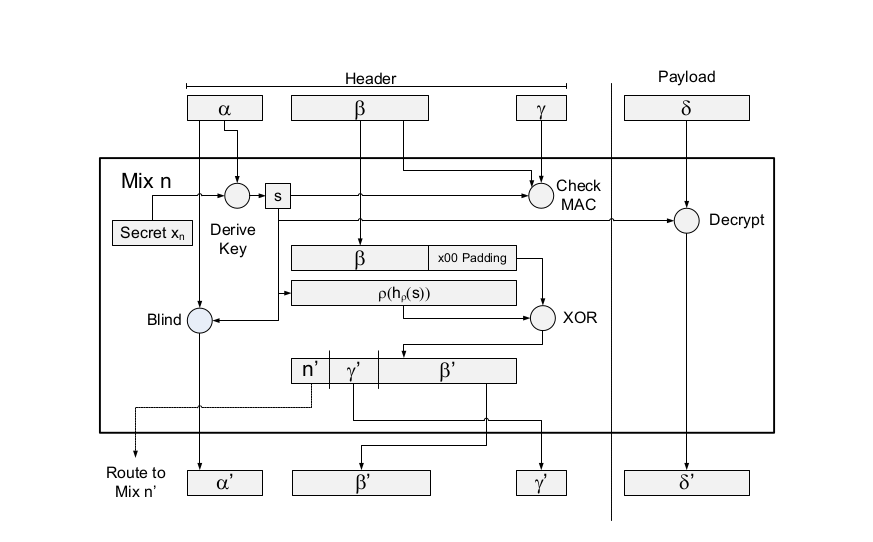
\includegraphics[width=11cm,height=11cm,keepaspectratio]{../yellowpaper/images/sphinx1.png}
    \caption{The processing of a Sphinx message \cite{sphinxpaper}}
    \label{fig:The processing of a Sphinx message }
\end{figure}
\hspace{-5mm}Same happens at $(C)$ and $(D)$: key derivation, unblinding, deleting, shifting, integrity check, decryption and blinding.
\subsection{Implementation choices}
Within HOPR, the following cryptographic primitives were used:
\begin{itemize}
    \item \textbf{Cyclic group:} The cyclic group used in the HOPR Sphinx implementation is an elliptic curve group on the secp256k1 curve and thus operations will be done on the elliptic curve.
    \item \textbf{Hash function:} BLAKE2s hash function which is a cryptographic hash function faster than SHA-2 and SHA-3, yet is at least as secure as SHA-3 and produces digests of any size between 1 and 32 bytes.
    \item \textbf{MAC:} HMAC based on a hash function BLAKE2s.
    \item \textbf{Encryption scheme:} LIONESS \cite{lionesspaper} implementation, using BLAKE2s as a hash function and ChaCha20 as a stream cipher.
    \item \textbf{Padding:} In the original SPHINX paper, a sequence of only 0s is used for padding, this allows the last mix-node in the path to infer information about the length of the path and the last destination, hence breaking one of the security properties promised by Sphinx. In order to prevent this attack, We replace the 0-padding by a randomized padding for the last exit-mix node and always take $v=r$. This way, the exit node can't identify where the padding starts and thus won't be able to find the path length that preceeds the padding.
\end{itemize}





